% Indicate the main file. Must go at the beginning of the file.
% !TEX root = ../main.tex

%----------------------------------------------------------------------------------------
% CHAPTER 5
%----------------------------------------------------------------------------------------

\chapter{Survey}

\label{Chapter5} % For referencing the chapter elsewhere, use \ref{Chapter2} 

In order to gain insight into potential adoption of these technologies, a survey was conducted among software engineering professionals. In total, 44 responses were collected from various teams and companies across diverse engineering domains. 
The questions and information provided in the survey are given in Appendix \ref{ApendixA}.

\section{Design of the survey}
The survey questions were designed to validate the various approaches employed by members of a Scrum team in order to enhance collaboration and productivity. The questions were grouped into four categories: participant demographics, role-specific information, decision logs within a mirrored approach, and \ac{IaC}. The concluding section of the survey comprises an additional optional question, which is designed to ascertain participants’ interpretations of potential combinations of tooling. It is anticipated that the responses to this question will assist in validating the approaches that were created on the basis of the four pillars of \ac{DevOps} outlined in chapter \ref{Chapter2} and developed in chapter \ref{Chapter4}, as well as any subsequent refinements. 

Furthermore, the questions aim to identify the challenges and limitations of the implementation process. This enables the development of enhanced approaches that are both resourceful and effective, and that are widely accepted by the team.


\pagebreak

\section{Demographics}

\subsection*{Gender}
The gender distribution of the survey participants is depicted in Figure \ref{fig:results:demo:1}. The majority of the respondents are male (90.9\%), with a smaller representation of females (6.8\%) and other genders (2.3\%). This distribution is indicative of the prevailing gender demographics within the software engineering sector, where male dominance is a well-documented phenomenon. While this imbalance reflects broader industry patterns, it also poses limitations on the diversity of insights gathered through this survey. The predominance of one gender may influence the survey's findings related to technology adoption and collaboration within \ac{SCRUM} teams, potentially skewing the results towards the perspectives and experiences more common among male engineers. Such a skew highlights the ongoing need for strategies aimed at enhancing diversity within the field, which could enrich innovation and the holistic understanding of team dynamics in technology-driven environments.


\begin{figure}[h!]
\centering
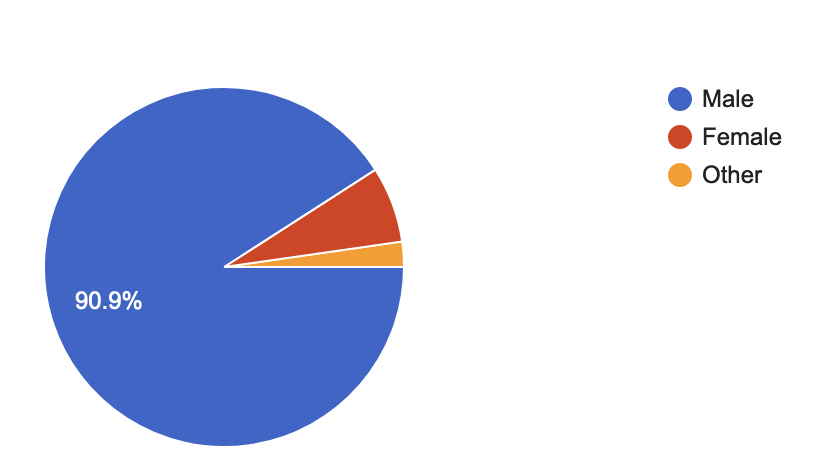
\includegraphics[width=\linewidth]{Images/Survey/demo_1.png}
\caption{Results for - Gender of the participants}
\label{fig:results:demo:1}
\end{figure}

\pagebreak

\subsection*{Your experience in the software engineering field?}

Figure \ref{fig:results:demo:2} presents the distribution of professional experience among the survey participants within the software engineering field. A substantial portion of the respondents, 50\%, possess over ten years of experience, highlighting the survey's capture of seasoned professionals' perspectives. An additional 22.7\% have precisely ten years of experience, further underscoring the experienced nature of the respondent pool. 

This predominance of experienced professionals suggests that the insights derived from this survey are grounded in extensive practical knowledge and awareness of the industry's evolution. However, the representation of those with five years or fewer (27.2\%) introduces a balance, potentially reflecting newer trends and adaptations in software engineering practices. This mixture of veteran and relatively newer engineers can provide a comprehensive overview of the current challenges and effective practices within the field, especially in relation to the adoption of new technologies and methodologies in software engineering.

\begin{figure}[h!]
\centering
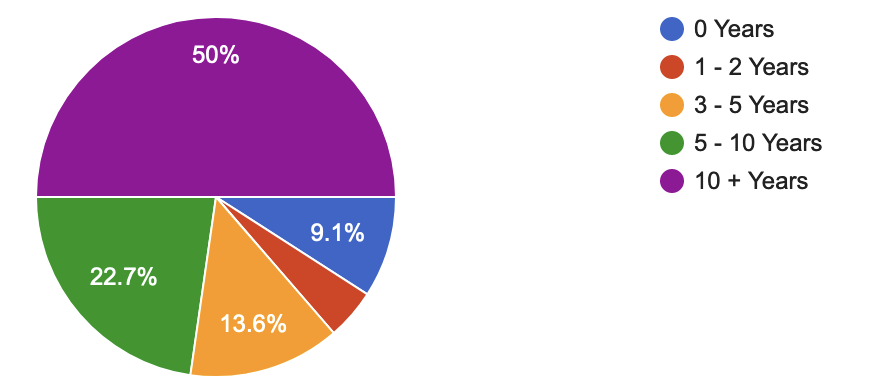
\includegraphics[width=\linewidth]{Images/Survey/demo_2.png}
\caption{Results for - Your experience in the software engineering field?}
\label{fig:results:demo:2}
\end{figure}

\pagebreak

\subsection*{Your level of education or training in software engineering?}
The survey assessed the educational background of the participants within the field of software engineering, revealing a diverse array of educational achievements as shown in Figure \ref{fig:results:demo:3}. The results indicate that 31.8\% of the participants hold a Master's degree or similar, and 29.5\% have a Bachelor's degree, underscoring a highly educated respondent base. Furthermore, a significant 25\% of the participants have gained their skills through self-education or training, reflecting the varied pathways into the software engineering profession.

This educational diversity suggests that the field not only attracts individuals with formal academic training but also those who are self-motivated to learn and adapt outside traditional educational frameworks. This mix of backgrounds may influence team dynamics and the adoption of new technologies, as individuals with different educational experiences might vary in their approaches to learning and integrating new tools. Additionally, the presence of formally trained individuals alongside self-taught professionals can enrich the collaborative environment, potentially leading to more innovative solutions and effective problem-solving within teams.


\begin{figure}[h!]
\centering
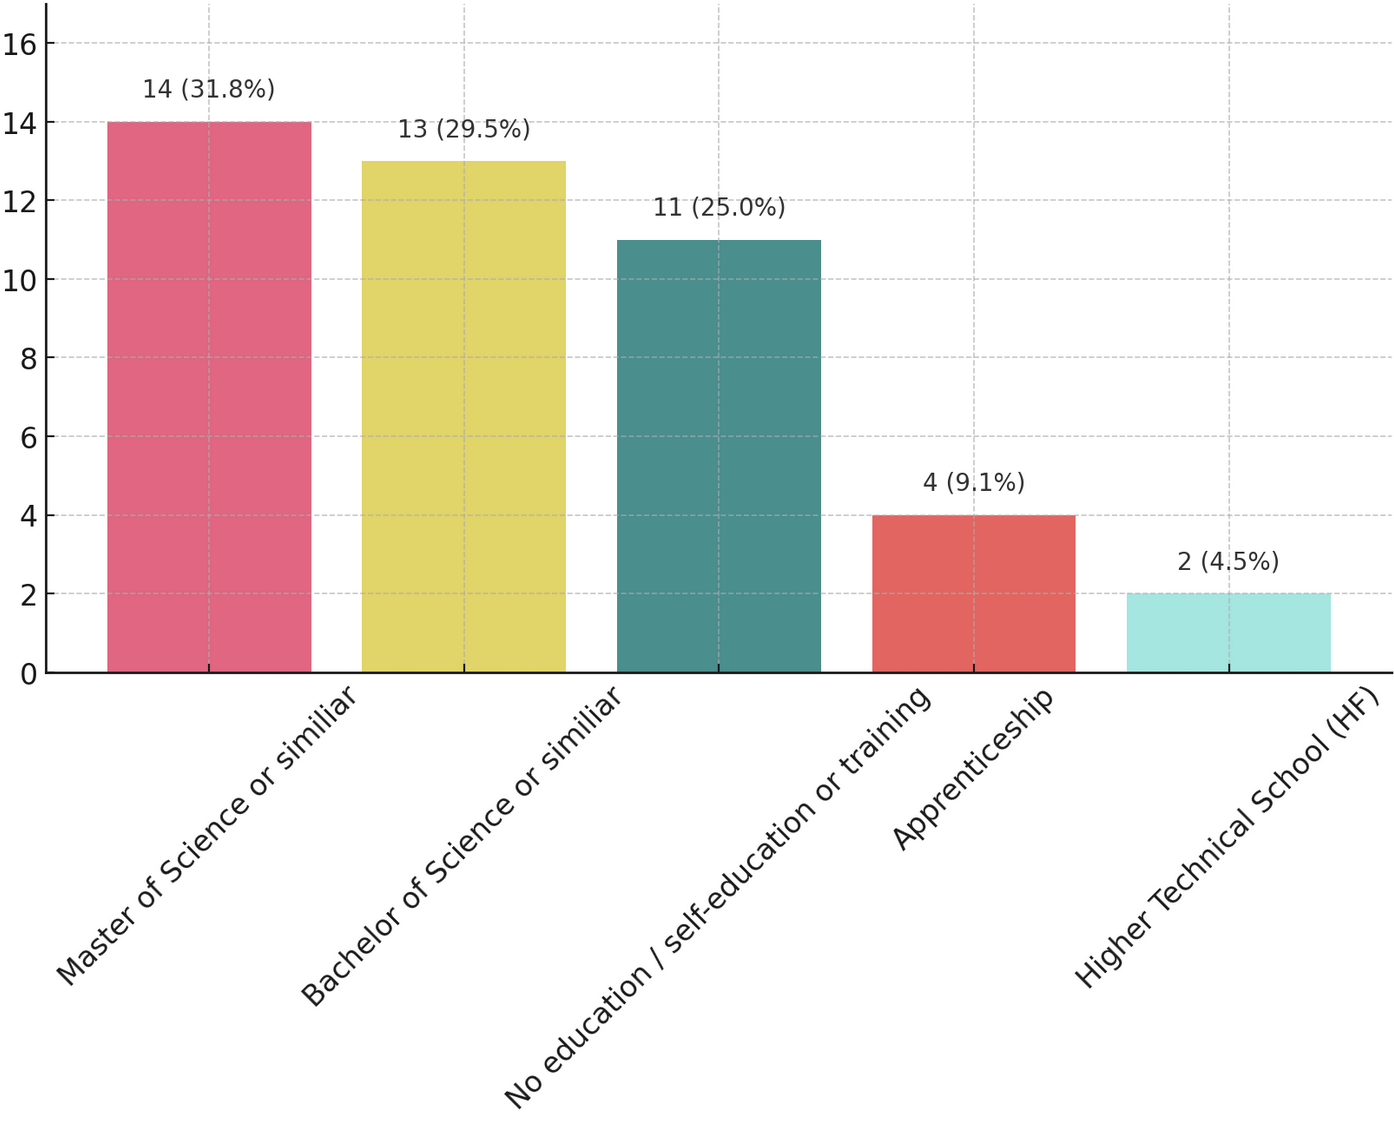
\includegraphics[width=\linewidth]{Images/Survey/demo_3.png}
\caption{Results for - Your level of education or training in software engineering?}
\label{fig:results:demo:3}
\end{figure}

\pagebreak

\subsection*{Your role in a software development team that best suits you.}
The survey assessed the preferred roles of participants within software development teams, showcasing a wide array of career focuses as depicted in Figure \ref{fig:results:demo:4}. The majority of respondents favor technical and design roles, with 29.5\% identifying as Developer/Engineer and 18.2\% as UI/UX Engineers, highlighting a strong inclination towards the foundational and creative aspects of software development.

Moreover, roles such as Project Owner (15.9\%) and QA Engineer (11.4\%) reflect the importance of leadership and quality assurance in software projects, underlining the multifaceted nature of team compositions required to meet today’s complex software development challenges. This diversity in role preference underscores the varied skill sets and perspectives that participants bring to their teams, potentially enriching collaboration and innovation.

The representation of roles across the spectrum from technical to strategic positions suggests that successful software development relies on a balanced integration of various expertises, with each role playing a critical part in the overall project lifecycle and contributing uniquely to the adoption of new technologies and methodologies.


\begin{figure}[h!]
\centering
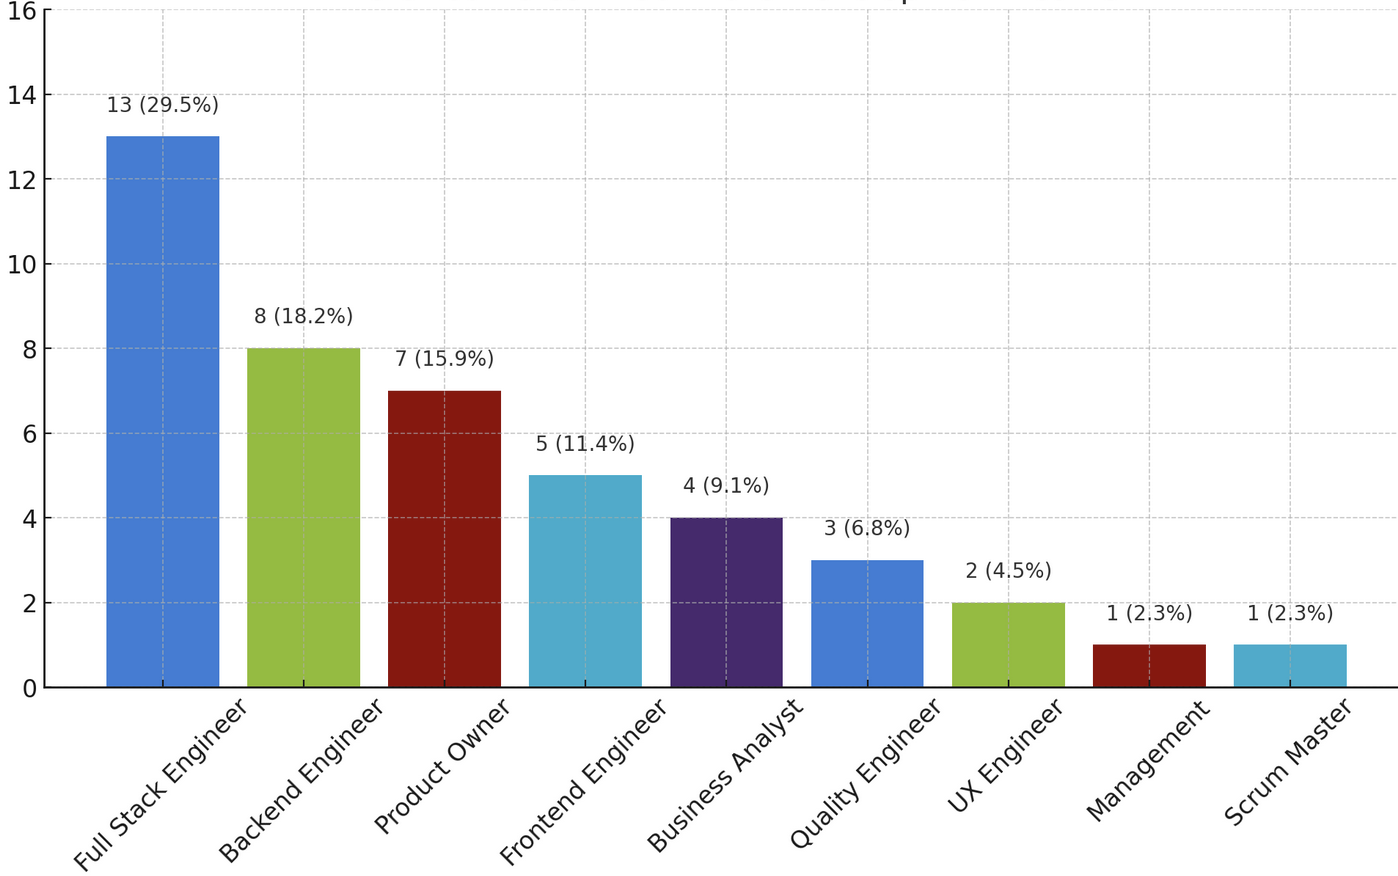
\includegraphics[width=\linewidth]{Images/Survey/demo_4.png}
\caption{Results for - Your role in a software development team that best suits you.}
\label{fig:results:demo:4}
\end{figure}

\pagebreak

\subsection*{Which software development paradigm is normally used in the projects you are involved with?}

The survey queried participants about their preferred software development paradigms, with the results indicating a strong inclination towards Agile and Extreme Programming (XP) methodologies. As illustrated in Figure \ref{fig:results:demo:5}, a significant majority of the participants (84.1\%) employ Agile/XP in their projects, underscoring its prominence in current software engineering practices. The remaining 15.9\% of respondents utilize a mixed approach, incorporating elements from various methodologies to suit specific project needs.

This predominant use of Agile/XP suggests that these methodologies continue to shape the landscape of software development, likely due to their effectiveness in managing complex projects and their adaptability to rapidly changing requirements. The minor yet notable preference for mixed methodologies also highlights a pragmatic approach to software development, where teams adapt and integrate different strategies to optimize outcomes.


\begin{figure}[h!]
\centering
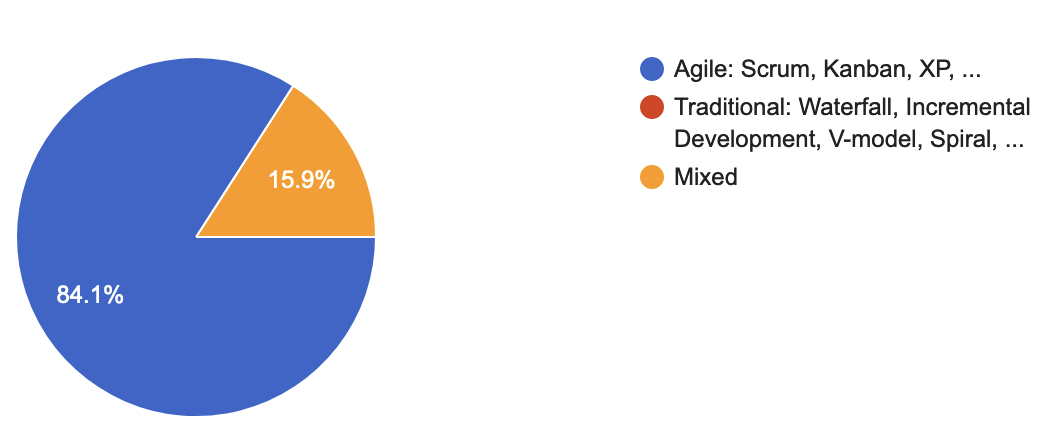
\includegraphics[width=\linewidth]{Images/Survey/demo_5.png}
\caption{Results for - Which software development paradigm is normally used in the projects you are involved with?}
\label{fig:results:demo:5}
\end{figure}

\pagebreak


\section{Role Based Information Highlighting in Documents}

\subsection*{Do you usually get overwhelmed by the amount of information when reading documentations?}
As shown in Figure \ref{fig:results:highlighting:1}, a significant number of respondents experience overwhelm with the volume of information in documentation. The highest frequencies are observed at the upper end of the scale, with 25\% of participants rating their level of overwhelm at 8, and 18.2\% at 7, indicating a notable discomfort. This trend underscores the necessity for improved information structuring and presentation in documentation to aid in better comprehension and usability for software engineering professionals. 


\begin{figure}[h!]
\centering
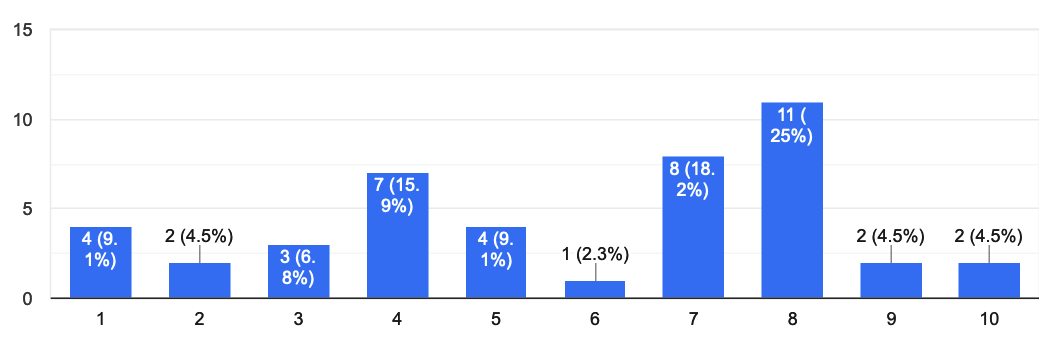
\includegraphics[width=\linewidth]{Images/Survey/documents_1.png}
\caption{Results for - Do you usually get overwhelmed by the amount of information when reading documentations?}
\label{fig:results:highlighting:1}
\end{figure}

\pagebreak

\subsection*{How satisfying would it be to have the information that is most important to you highlighted for you?}
Figure \ref{fig:results:highlighting:2} illustrates a strong positive response to the idea of having key information highlighted in documentation. The majority of the respondents (75\%) expressed high satisfaction (ratings of 8 to 10), highlighting the potential benefit and demand for such features in documentation tools. This response underscores the importance of adaptive and user-centric information presentation, which could significantly enhance readability and efficiency in professional settings.

\begin{figure}[h!]
\centering
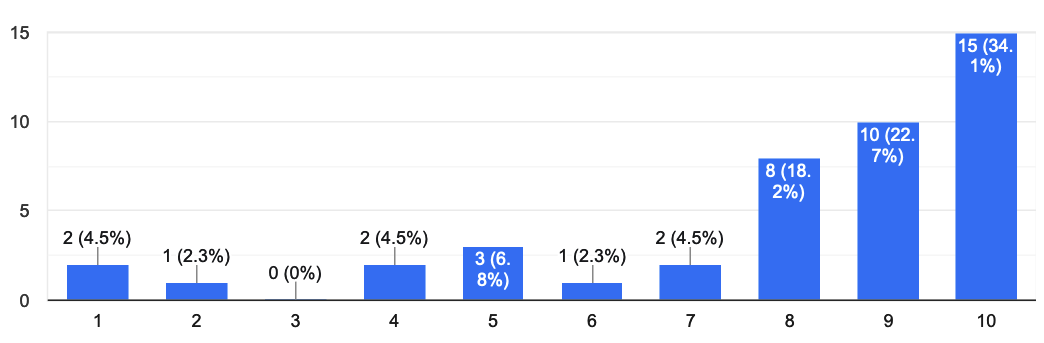
\includegraphics[width=\linewidth]{Images/Survey/documents_2.png}
\caption{Results for - How satisfying would it be to have the information that is most important to you highlighted for you?}
\label{fig:results:highlighting:2}
\end{figure}

\pagebreak


\subsection*{How easy do you think it would be to use \ac{AI} to automate the highlighting of information based on a viewer's role selection?}
Figure \ref{fig:results:highlighting:3} displays a diverse range of opinions regarding the ease of using \ac{AI} for automated information highlighting. The data shows a notable spread across the scale with a concentration in the moderate-to-high feasibility range (ratings of 6 to 7), indicating a cautious optimism. This suggests a recognition of \ac{AI}'s potential, paired with an awareness of the practical and technical challenges that might be encountered. The mixed responses underscore the need for ongoing research and development to enhance \ac{AI}'s capabilities and ease of integration into existing workflows, especially in complex fields such as software engineering.

\begin{figure}[h!]
\centering
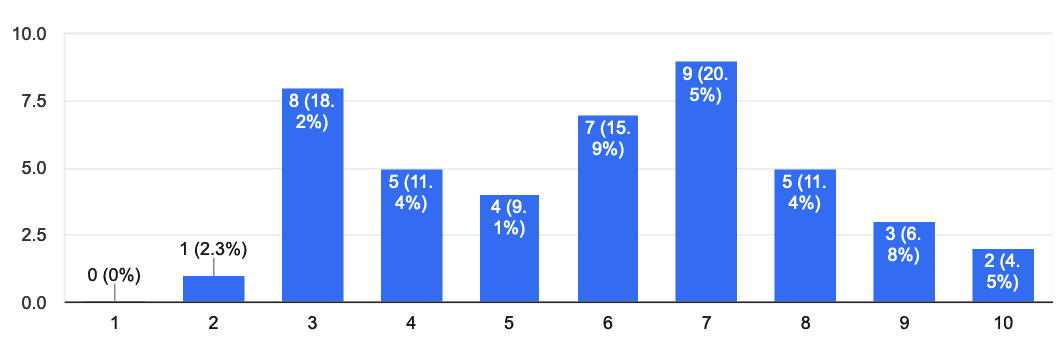
\includegraphics[width=\linewidth]{Images/Survey/documents_3.png}
\caption{Results for - How easy do you think it would be to use \ac{AI} to automate the highlighting of information based on a viewer's role selection?}
\label{fig:results:highlighting:3}
\end{figure}

\pagebreak

\subsection*{How much better do you think this approach of highlighting just the right information is than having separate pages for different roles?}
Figure \ref{fig:results:highlighting:4} illustrates a positive reception towards the highlighting approach over having separate pages for different roles. A majority of respondents (59.1\%) rated the benefit of this approach as high (7 to 10 on the scale), underscoring the perceived efficiency and effectiveness of integrating information in a single document with role-specific highlights. This preference highlights the potential for tools that can intelligently adapt content presentation to user needs, enhancing usability and accessibility in professional settings. However, a significant proportion of participants showed some reservations, indicating a need for further exploration into the implementation challenges and accuracy of such \ac{AI}-driven solutions.
\begin{figure}[h!]
\centering
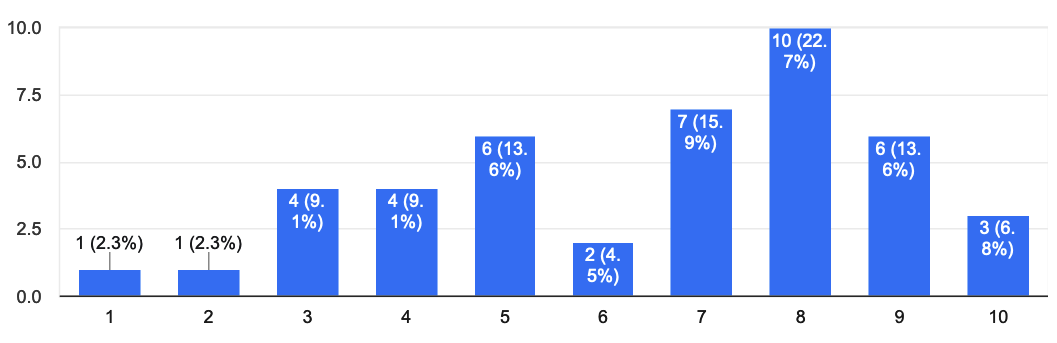
\includegraphics[width=\linewidth]{Images/Survey/documents_4.png}
\caption{Results for - How easy do you think it would be to use \ac{AI} to automate the highlighting of information based on a viewer's role selection?}
\label{fig:results:highlighting:4}
\end{figure}

\pagebreak

\subsection*{In your personal experience, do you see people using more text or screenshots to document information?}
Figure \ref{fig:results:highlighting:5} depicts a varied spectrum of preferences between text and screenshots in documentation practices. A substantial number of participants lean towards a balanced or slightly higher use of screenshots (scale points 4 to 8), indicating a preference for visual documentation elements in certain contexts. This suggests that while traditional text-based documentation remains foundational, the integration of visual elements like screenshots is becoming increasingly prevalent, possibly due to their ability to convey complex information more effectively and engagingly. This trend underscores the need for tools and practices that seamlessly integrate both textual and visual information to accommodate diverse documentation needs and preferences.

\begin{figure}[h!]
\centering
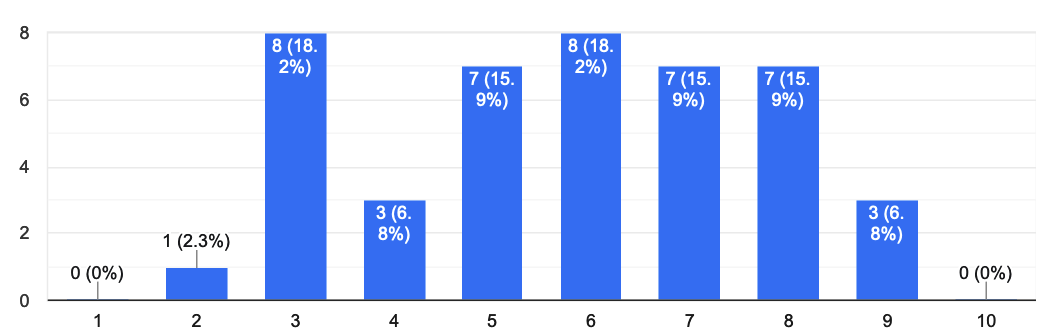
\includegraphics[width=\linewidth]{Images/Survey/documents_5.png}
\caption{Results for - In your personal experience, do you see people using more text or screenshots to document information?}
\label{fig:results:highlighting:5}
\end{figure}

\pagebreak

\section{Decision Logs Within a Mirrored Approach}

\subsection*{How important do you think it is to have a record of decisions and an up-to-date record of decisions?}
Figure \ref{fig:results:decisions:1} illustrates a strong consensus among participants on the importance of maintaining a thorough and current record of decisions. A significant majority (70.5\%) rated this necessity highly (8 to 10 on the scale), highlighting the critical role that decision logs play in ensuring transparency, continuity, and accountability in organizational processes. This strong endorsement underlines the need for robust systems and practices that can reliably document and update decision records, serving as a foundational aspect of effective project management and operational efficiency.

\begin{figure}[h!]
\centering
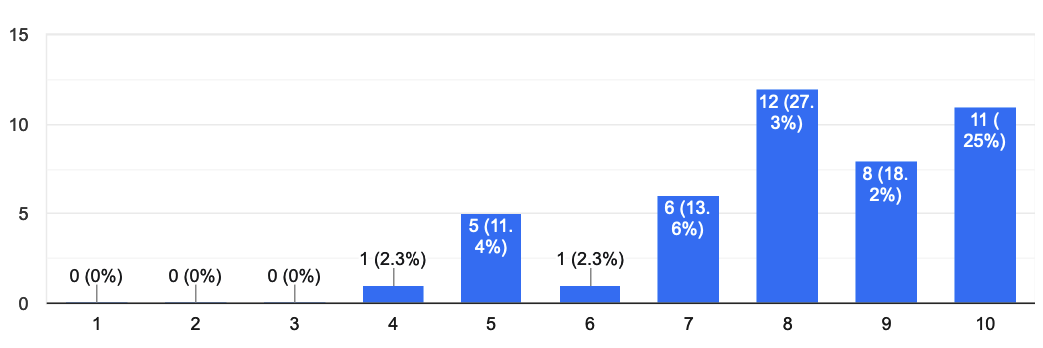
\includegraphics[width=\linewidth]{Images/Survey/decisions_1.png}
\caption{Results for - How important do you think it is to have a record of decisions and an up-to-date record of decisions?}
\label{fig:results:decisions:1}
\end{figure}

\pagebreak

\subsection*{Did the decision logs you've seen so far contain the most up-to-date information, were they properly formatted and did they make sense?}
Figure \ref{fig:results:decisions:2} presents a mixed response to the quality of decision logs encountered by participants. While a small segment of respondents (29.5\%) expressed relatively high satisfaction (ratings 7 to 10), the majority (65.9\%) rated their experience with decision logs as average to poor (ratings 1 to 6). This underscores a critical need for improvements in how decision logs are maintained and formatted. Ensuring that decision logs are up-to-date, clear, and logically structured is paramount to their utility in guiding and documenting project decisions effectively.

\begin{figure}[h!]
\centering
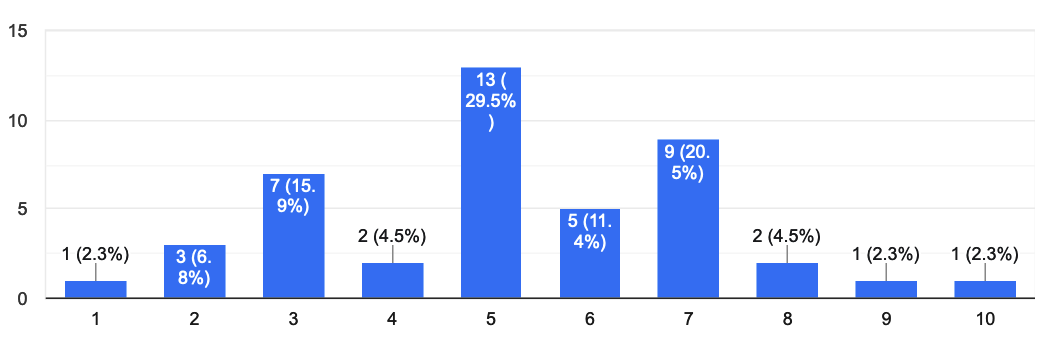
\includegraphics[width=\linewidth]{Images/Survey/decisions_2.png}
\caption{Results for - Did the decision logs you've seen so far contain the most up-to-date information, were they properly formatted and did they make sense?}
\label{fig:results:decisions:2}
\end{figure}

\pagebreak

\subsection*{How do you think the decision logs would benefit from being part of the relevant code base, rather than a separate document, in terms of being up to date?}
Figure \ref{fig:results:decisions:3} reveals a strong preference among participants for integrating decision logs directly within the code base. The majority of respondents (68\%) perceive high benefits (ratings 7 to 10) from such integration, emphasizing its potential to keep decision records more current and closely tied to the actual code changes they pertain to. This approach could enhance the accuracy and timeliness of decision logs, making them more dynamic and immediately relevant. However, a considerable minority expressed reservations, highlighting the need for careful consideration of implementation strategies to address potential barriers and optimize usability for all stakeholders.

\begin{figure}[h!]
\centering
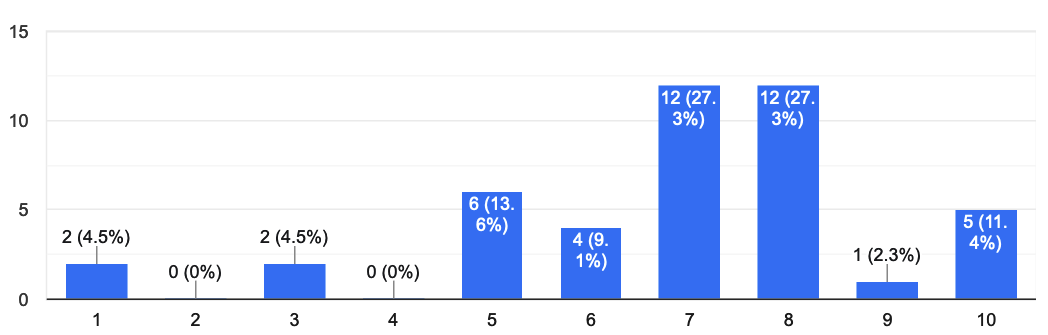
\includegraphics[width=\linewidth]{Images/Survey/decisions_3.png}
\caption{Results for - How do you think the decision logs would benefit from being part of the relevant code base, rather than a separate document, in terms of being up to date?}
\label{fig:results:decisions:3}
\end{figure}

\pagebreak

\subsection*{How important do you think it is, if the decision logs are in the associated codebase, to still keep them in a document accessible to "non-developers"?}
Figure \ref{fig:results:decisions:4} demonstrates a significant valuation of making decision logs accessible to non-developers, with over half of the respondents (52.3\%) rating this importance highly (8 to 10). This underlines the perceived need for transparency and inclusivity in project documentation, facilitating broader understanding and engagement across all stakeholders. However, nearly half of the participants expressed less concern, highlighting diverse views on the operational and security challenges of broadly accessible decision logs. This dichotomy suggests a need for balanced solutions that cater to the needs of diverse project teams while ensuring that decision logs remain comprehensible and secure.

\begin{figure}[h!]
\centering
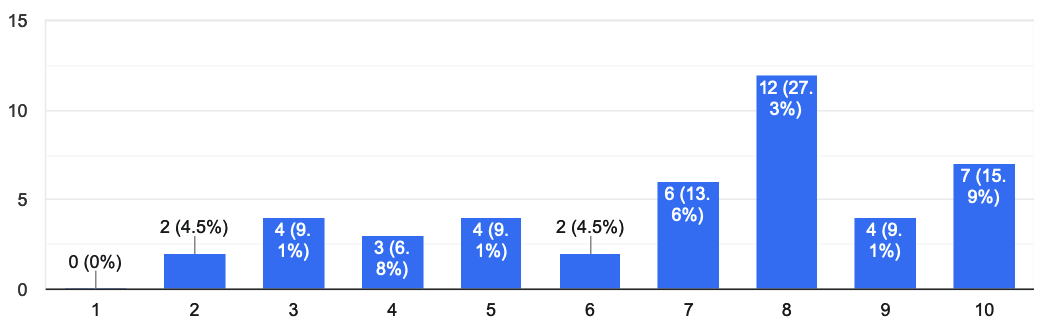
\includegraphics[width=\linewidth]{Images/Survey/decisions_4.png}
\caption{Results for - How important do you think it is, if the decision logs are in the associated codebase, to still keep them in a document accessible to "non-developers"?}
\label{fig:results:decisions:4}
\end{figure}

\pagebreak


\subsection*{How easy do you think it would be to use tools to automate the mirroring of decisions into a separate document accessible to everyone?}
Figure \ref{fig:results:decisions:5} indicates a wide range of opinions regarding the ease of using tools to automate the mirroring of decision logs. While a moderate number of respondents (52.3\% with ratings 4 to 7) believe that it is reasonably feasible, a significant portion (29.5\% with ratings 1 to 3) express reservations, suggesting perceived complexities or usability issues with existing tools. On the other hand, a smaller segment (18.2\% with ratings 8 to 10) shows strong confidence in the current capabilities of such tools. This spread of responses highlights the need for further research into tool development, focusing on enhancing user-friendliness and integration capabilities to support effective decision log management across diverse teams.

\begin{figure}[h!]
\centering
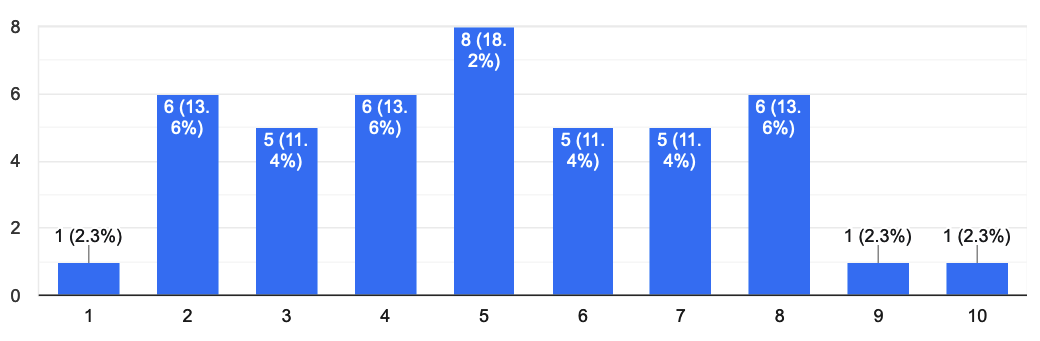
\includegraphics[width=\linewidth]{Images/Survey/decisions_5.png}
\caption{Results for - How easy do you think it would be to use tools to automate the mirroring of decisions into a separate document accessible to everyone?}
\label{fig:results:decisions:5}
\end{figure}

\pagebreak


\section{Infrastructure as Code}

\subsection*{In your current software project, how much do you know about how deployments and architectures work?}
Figure \ref{fig:results:iac:1} reflects varied levels of understanding among participants regarding the deployments and architectures in their software projects. Nearly half of the respondents (47.7\%) report high knowledge (ratings of 8 to 10), showcasing a strong command over technical aspects of their projects. This level of proficiency is crucial for effective project management and could potentially influence the adoption and success of \ac{IaC} practices. Meanwhile, the substantial number of moderate responses (38.6\%) signals areas where targeted educational initiatives could further enhance team capabilities and project outcomes.

\begin{figure}[h!]
\centering
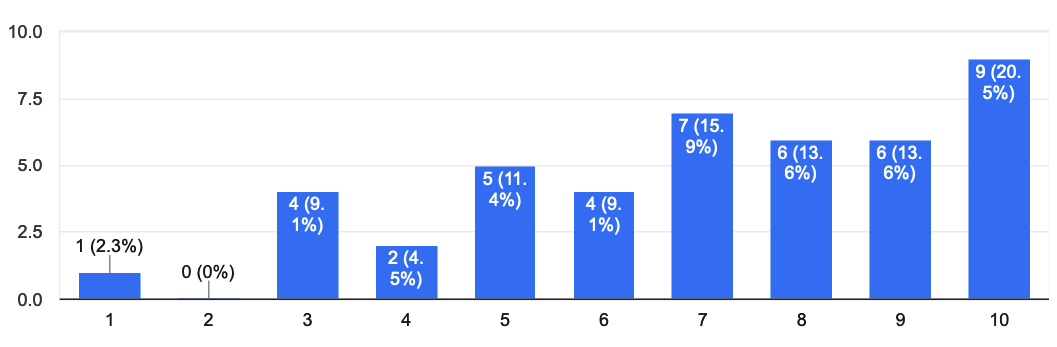
\includegraphics[width=\linewidth]{Images/Survey/iac_1.png}
\caption{In your current software project, how much do you know about how deployments and architectures work?}
\label{fig:results:iac:1}
\end{figure}

\pagebreak


\subsection*{How familiar are you with the concept of IaC and its benefits?}
Figure \ref{fig:results:iac:2} illustrates a wide spectrum of familiarity with the concept of \ac{IaC} among the survey participants. Notably, a significant portion of the respondents (38.6\%) possess limited knowledge of \ac{IaC}, as indicated by the low ratings (1 to 4). This suggests a potential barrier to the full adoption and optimization of \ac{IaC} practices within their projects. On the other hand, nearly 30\% of the participants demonstrate a high understanding (ratings of 8 to 10), which could indicate a readiness to implement or enhance \ac{IaC} solutions effectively. The results underscore the need for targeted educational programs that could bridge the knowledge gap and facilitate a deeper understanding and utilization of \ac{IaC} benefits across software teams.
\begin{figure}[h!]
\centering
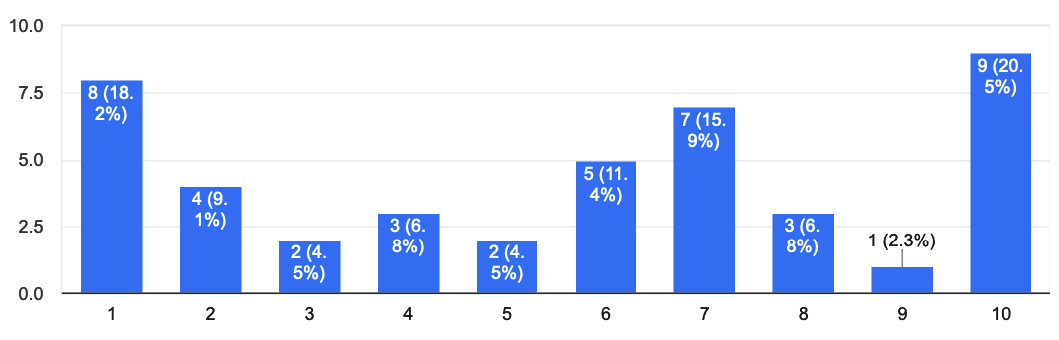
\includegraphics[width=\linewidth]{Images/Survey/iac_2.png}
\caption{How familiar are you with the concept of IaC and its benefits?}
\label{fig:results:iac:2}
\end{figure}

\pagebreak

\subsection*{To what extent do you agree that IaC helps in fostering a sense of shared responsibility among development team members?}

Figure \ref{fig:results:iac:3} indicates a predominantly positive reception to the role of \ac{IaC} in fostering shared responsibility among team members, with over half of the respondents (52.3\%) expressing high agreement (ratings 7 to 10). This response suggests that \ac{IaC} is viewed not only as a technical tool but also as a facilitator of collaborative and accountable practices within development teams. However, a significant proportion of participants (36.4\%) provided moderate responses, highlighting potential variability in experiences or perceptions of \ac{IaC}'s effectiveness in this regard. This mixed response underscores the need for further investigation into how \ac{IaC} practices are implemented and perceived across different team environments and project contexts.

\begin{figure}[h!]
\centering
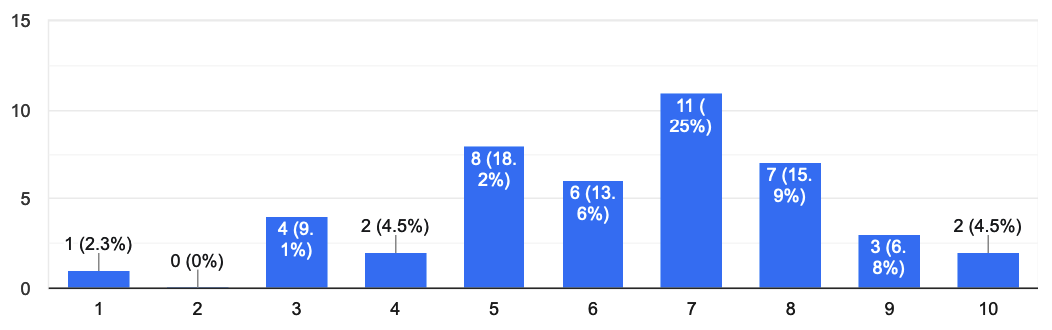
\includegraphics[width=\linewidth]{Images/Survey/iac_3.png}
\caption{To what extent do you agree that IaC helps in fostering a sense of shared responsibility among development team members?}
\label{fig:results:iac:3}
\end{figure}

\pagebreak

\subsection*{What are the biggest challenges or limitations you have faced when implementing IaC in your projects?}
The survey elicited detailed feedback on the challenges faced by software engineering professionals when implementing \ac{IaC}. As depicted in the responses, a significant range of obstacles impacts the adoption and effective use of \ac{IaC} technologies.

\textbf{Complexity and Knowledge Gaps:} Respondents highlighted the inherent complexity involved in managing and understanding intricate infrastructure configurations, particularly in larger-scale projects. This complexity is exacerbated by gaps in necessary skills, with several participants noting the steep learning curve associated with mastering domain-specific configuration languages and tools like Terraform.

\textbf{Migration and Adaptation:} Legacy systems pose substantial challenges, with their migration to \ac{IaC} described as particularly difficult. Issues in modifying existing, often poorly structured configuration files further complicate transitions to \ac{IaC} practices.

\textbf{Team Dynamics and Expertise Concentration:} A recurring theme in the responses was the concentration of \ac{IaC} knowledge within small subsets of teams, leading to knowledge silos and dependency on few individuals. This situation poses risks in knowledge continuity and creates barriers for broader team involvement.

\textbf{Security and Operational Risks:} Security emerged as a critical concern, with respondents expressing worries about accidentally exposing resources due to misconfigurations. The operational challenges of testing and rapidly adapting \ac{IaC} configurations in dynamic environments were also noted as significant hurdles.

These insights underline the need for comprehensive strategies to enhance training, improve documentation and knowledge sharing, and foster more inclusive team involvement in \ac{IaC} practices to mitigate these challenges effectively.


\section{Summary}

\subsection*{In your opinion, what combination of techniques would be the most effective?}

This question sought to identify which combinations of development techniques are perceived as the most effective by participants. The results highlight a clear preference for integrating specific approaches to enhance the overall software development process.

\begin{itemize}
    \item \textbf{Role-Based Information Highlighting + Decision Logs Mirroring:} This combination received the most endorsements, with 12 participants highlighting its effectiveness. The integration of role-based information highlighting with mirrored decision logs likely offers significant improvements in ensuring that all team members have access to the necessary information in a format that supports effective decision-making and accountability.

    \item \textbf{Decision Logs Mirroring + Infrastructure as Code:} With 9 votes, this pairing underscores the value of maintaining transparent and traceable changes within automated infrastructure setups, suggesting that decision logs mirroring complements the precision and automated nature of IaC.

    \item \textbf{Infrastructure as Code + Role-Based Information Highlighting:} Although it received fewer votes (7 participants), the combination of tailored information delivery with automated infrastructure management is recognized as beneficial, particularly for managing complex environments efficiently and accurately.
\end{itemize}


%----------------------------------------------------------------------------------------